\documentclass[11pt]{article}
\usepackage{graphicx}
\usepackage{times}
\usepackage{amssymb}
\usepackage{float}
\usepackage{amsmath,amssymb,amsfonts,bm}

\newcount\refno\refno=1
\def\ref{\the\refno \global\advance\refno by 1}
\def\ux{\underline{x}}
\def\uw{\underline{w}}
\def\ut{\underline{\theta}}
\def\umu{\underline{\mu}}
\def\be{p_e^*}
\newcount\eqnumber\eqnumber=1
\def\eq{\the \eqnumber \global\advance\eqnumber by 1}
\def\eqs{\eq}
\def\eqn{\eqno(\eq)}

 \pagestyle{empty}
\def\baselinestretch{1.1}
\topmargin1in \headsep0.3in
\topmargin0in \oddsidemargin0in \textwidth6.5in \textheight8.5in
\begin{document}
\setlength{\parskip}{1.2ex plus0.3ex minus 0.3ex}


\thispagestyle{empty} \pagestyle{myheadings} \markright{Homework
3: CS 274A, Probabilistic Learning: Winter 2019}



\title{CS 274A Homework 3}
\author{Caleb Nelson}
\date{Due Date:  11am  Monday February 4th}


\maketitle


\section*{Instructions and Guidelines for Homeworks}
 \begin{itemize}

\item
Please answer all of the questions and submit a scanned copy of your written solutions to Gradescope 
(either hand-written or typed are fine as long as the writing is legible). 
%Code (if requested) should be submitted to the EEE dropbox. No
%need to submit any code unless we request it.

\item
All problems are worth 10 points unless otherwise stated.  All homeworks will get equal weight in computation of the final grade for the class.
 \item
The homeworks are intended to help you work through the concepts
we discuss in class in  more detail. It is important that you try
to solve the problems yourself. The homework problems are important to help you better
learn and reinforce the material from class. If you don't
do the homeworks you will likely have difficulty in the exams
later in the quarter.

\item If you can't solve a
problem, you can discuss it {\it verbally} with another student. However, please note that before you submit your homework solutions you
are not allowed to view (or show to any other student) any {\it written material} directly related to the homeworks, including other students' solutions or drafts of solutions, solutions from previous versions of this class, and so forth. The work you hand in should be your own original work.

\item You are allowed to use reference materials in your solutions, such as class notes, textbooks,  other reference material (e.g., from the Web), or solutions to other problems in the homework. It is strongly recommended that you first try to solve the problem yourself, without resorting to looking up solutions elsewhere. If you base your solution on material that we did not discuss in class, or is not in the class notes, then you need to clearly provide a reference, e.g., ``based on material in Section 2.2 in ....."


\item
In problems that ask for a proof you should submit a complete mathematical
proof (i.e., each line must follow logically from the preceding one, without
``hand-waving"). Be as clear as possible in explaining
 your notation and in stating your reasoning as you go from line to line.  


\item
If you wish to use LaTeX to write up
your solutions you may find it useful to use the .tex file for  this homework
that is posted on the Web page. 






\end{itemize}

\subsection*{Problem \ref: Properties of the Beta Density}
In class we will discuss the use of a Beta density function as a prior density for a parameter that lies between 0 and 1. The Beta density is defined as:
\begin{equation}
P(\theta) \ = \ Be(\theta; \alpha, \beta)  \ = \  \frac{1}{B(\alpha,\beta)}  \theta^{\alpha-1} (1 - \theta)^{\beta-1}
\end{equation}
where $0 \le \theta \le 1$. The two parameters of this density function are $\alpha>0$ and $\beta>0$ and $B(\alpha,\beta)$ is a normalization constant to ensure that the density integrates to 1, where
$B(\alpha,\beta) = \frac{\Gamma(\alpha)\Gamma(\beta)}{\Gamma(\alpha + \beta)}$ and $\Gamma(z) = \int_0^{\infty} x^{z-1} e^{-x} dx$, $z > 0$, is the gamma function. 

In solving the problems below keep in mind that since $B(\alpha,\beta)$ is the normalization constant for the density, then by definition $\frac{1}{B(\alpha,\beta)} = \int_0^1 \theta^{\alpha-1} (1 - \theta)^{\beta-1} d\theta$. Another useful fact  that the gamma function has the property that $\Gamma(z+1) = z \Gamma(z)$.
\begin{enumerate}
\item
Derive an expression  for  the mean of a Beta density, as a function of the parameters $\alpha$ and $\beta$.

\begin{multline}
	\mu = E[X] = \int_0^1 xf(x;\alpha,\beta)dx = 
	\int_0^1 x\frac{x^{\alpha-1}(1-x)^{\beta-1}}{B(\alpha,\beta)}dx = \\
	\int_0^1 x^\alpha(1-x)^{\beta-1}dx * \int_0^1 \frac{1}{B(\alpha,\beta)}dx = \\
	\int_0^1 x^\alpha(1-x)^{\beta-1}dx * 1 = \frac{\alpha}{\alpha + \beta}
\end{multline}

\item
 Derive an expression  for the mode of a Beta density, as a function of the parameters $\alpha$ and $\beta$. You can assume in this case that $\alpha>1$ and $\beta>1$.

The mode is arrived at by setting the deriviation of the pdf to zero so
\begin{equation}
	\frac{d}{dx} \frac{x^{\alpha-1}(1-x)^{\beta-1}}{B(\alpha,\beta)} = 
	\frac{(\alpha-1)x^{\alpha-2}(1-x)^{\beta-1}-(\beta-1)x^{\alpha-1}(1-x)^{\beta-2}}{B(\alpha,\beta)}
\end{equation}
Setting this equal to 0 and solving for x gives us
\begin{multline}
	(\alpha-1)x^{\alpha-2}(1-x)^{\beta-1}-(\beta-1)x^{\alpha-1}(1-x)^{\beta-2} = 0 \\ 
	(\alpha-1)(1-x) - x(\beta-1) = 0 \\ 
	\alpha-\alpha x-1+x-x\beta+x = 0 \\
	x(2-\alpha-\beta) = 1-\alpha \\
	x = \frac{\alpha-1}{\alpha+\beta-2}
\end{multline}

\end{enumerate}
 

 
% Bayesian estimation with the Dirichlet-Multinomial model

\subsection*{Problem \ref: (Bayesian Estimation for the Multinomial Model)}

Consider a data set $D = \{x_1,\ldots,x_N\}$, with $x_i \in \{1, \ldots, M\}$ where the $x_i$'s are independent draws from a discrete-valued distribution with parameters $\theta_k = P(x_i = k), 1 \le k \le M$, and $\sum_{k=1}^M \theta_k = 1$ (i.e., we have a multinomial likelihood for the $x_i$'s). Assume that we have a Dirichlet prior for the parameters $\theta$, where the prior has parameters $\alpha_1,\ldots,\alpha_M$ and $ \alpha_k > 0$ and $1 \le k \le M$.
\begin{enumerate}
\item Prove that the posterior distribution on $\theta_1,\ldots,\theta_K$ is also Dirichlet.

The posterior is proportional to the prior times the likelihood, which for this is
\begin{equation}
	\prod_{i=1}^N \theta_i^{r_i} * \prod_{i=1}^N \theta_i^{\alpha_i - 1} = 
	\prod_{i=1}^N \theta_i^{\alpha_i + r_i - 1}
\end{equation}
where $r_i$ is the number of data points equal to $i$ in $D$. 
This is equivalent to a Dirichlet distribution with parameters 
$(\alpha_1 + r_1, ..., \alpha_M + r_M)$.

\item Derive an expression for the maximum a posteriori (MAP) estimate for  $\theta_k, 1 \le k \le M$. Your solution should be derived from first principles (i.e. using basic calculus to find the mode of the posterior density for $\theta_k$, working from your solution for
 $P(\theta | D)$ from part 1).

\begin{equation}
	\frac{d}{d\theta_k} \prod_{i=1}^N \theta_i^{\alpha_i + r_i - 1} = 
	(a_k+r_k-1)\theta_k^{a_k+r_k-2} \prod_{i=1, i\neq k}^N \theta_i^{\alpha_i + r_i - 1}
\end{equation}
Setting this equal to 0 and solving for $\theta_k$ gives us
\begin{equation}
	\frac{\alpha_k + r_k - 1}{\sum_{m=1}^M \alpha_m - M}
\end{equation}
for the mode. This mode is equal to the MAP estimate for $\theta_k$

\end{enumerate}

\subsection*{Problem \ref: (Bayesian Estimation of a Gaussian Model)}

For the case of the mean $\mu$ of a Gaussian model, with known variance $\sigma^2$, and
with a Gaussian prior on $\mu$ that has mean $\mu_0$ and variance $s^2$, we discussed in class
the fact that the posterior density for $\mu$, given $n$ IID observations $\{x_1,\ldots,x_n\}$
is also Gaussian with parameters $\mu_n$ and $\sigma^2_n$. Prove that the following expressions for  the
mean of this posterior and the variance of this posterior are correct, i.e.,
\[
\mu_n \ = \ \gamma \hat{\mu}_{ML}  \ + \ (1-\gamma) \mu_0
\]
where
\[
\gamma = \frac{n s^2}{n s^2 + \sigma^2}.
\]
and
\[
\frac{1}{\sigma_n^2} = \frac{n}{\sigma^2} + \frac{1}{s^2}
\]

The posterior density for $\mu$ is proportional to
\begin{equation}
	\frac{e^{-\frac{(\mu-\mu_0)^2}{2s^2}}}{\sqrt{2\pi s^2}} * 
	\frac{e^{-\frac{\sum_{i=1}^n (x_i - \mu)^2}{2\sigma^2}}}{(2\pi \sigma^2)^{n/2}} = 
	\frac
		{e^{\frac{-\mu^2 + 2\mu\mu_0 - \mu_0^2}{2s^2} - \sum_{i=1}^n \frac{x_i^2 - 2x_i\mu + \mu^2}{2\sigma^2}}}
		{(2\pi)^\frac{n+1}{2} \sqrt{s^2 \sigma^{2n}}}
\end{equation}
The denominator of this fraction is constant with respect to $\mu$, so it can wrapped up in the normalization term. Doing so leaves us with
\begin{multline}
	e^{\frac{-\mu^2 + 2\mu\mu_0 - \mu_0^2}{2s^2} - \sum_{i=1}^n \frac{x_i^2 - 2x_i\mu + \mu^2}{2\sigma^2}} = 
	e^{\frac{-\mu^2(\sigma^2 + ns^2) + 2\mu(\mu_0\sigma^2 + s^2x+1 + ... + s^2) - (\mu_0^2\sigma^2 + s^2 x_1^2 + ... + s^2 x_n^2)}{2s^2\sigma^2}} \\
	= e^{-\frac{(\mu - \frac{\mu_0\sigma^2 + \sum_{i=1}^n s^2 x_i}{\sigma^2 + ns^2})^2}{2\frac{s^2\sigma^2}{\sigma^2 + ns^2}}}
\end{multline}
While hard to read, this expression is in fact the PDF of a gaussian with parameters
\begin{equation}
	\sigma_n^2 = \frac{s^2\sigma^2}{\sigma^2 + ns^2} = \frac{1}{s^{-2}+n\sigma^{-2}}, 
	\frac{1}{\sigma_n^2} = \frac{1}{s^2} + \frac{n}{\sigma^2}
\end{equation}
and
\begin{equation}
	\mu_n = \frac{\mu_0\sigma^2 + \sum_{i=1}^n s^2 x_i}{\sigma^2 + ns^2}
	\frac{}{}
\end{equation}
which is equivalent to the stated definition for $\mu_n$


\subsection*{Problem \ref: (Bayesian Estimation for the Geometric Model)}
Let $X$ be a geometric random variable taking values $x \in \{0, 1, 2, \ldots\}$, with probability distribution defined as
\begin{equation}
P(x) \ = \ (1-\theta)^x \theta, \ \ \ \ \ \mbox{for} \ x = 0,1,2,\ldots
\end{equation}
where $\theta$ is the parameter of the geometric model and $0 < \theta < 1$.   The geometric distribution models a problem  where we have a sequence of random binary outcomes with ``success" probability $\theta$, where the outcomes are generated independently at each step, and $x$ is the number of steps before success. For example this could be a model of the number of tails we see in tossing a coin before we see heads, where $\theta$ is the probability of heads.

Let $D = \{x_1,\ldots,x_N\}$ be an observed data set where we assume the samples were generated in an IID manner from $P(x)$. 
\begin{enumerate}
\item Define the likelihood function for this problem. \\
The likelihood function for the geometric model is $L(\theta | x_1, ..., x_n) = \prod_i^n P(x_i | \theta) = \theta^n(1-\theta)^{\sum_i^n x_i}$

\item Prove that the Beta density $Be(\alpha,\beta)$ is a conjugate prior for the Geometric likelihood and derive an equation for the posterior density for $\theta$. (A prior is said to be {\it conjugate} to a particular type of likelihood function  whenever the posterior has the same functional form (the same type of density) as the prior).
\begin{equation}
	P(\theta)P(D|\theta) \propto \theta^{\alpha-1}(1-\theta)^{\beta-1} * \theta^n(1-\theta)^{\sum_i^n x_i} = 
	\theta^{\alpha+n-1}(1-\theta)^{\beta+\sum_i^n x_i - 1}
\end{equation}
This is a beta distribution with parameters $(\alpha+n, \beta+\sum_i^n x_i)$.
This is the posterior density for $\theta$, and since it is also a beta distribution, $Be(\alpha, \beta)$ 
is a conjugate prior for the geometric likelihood.

\end{enumerate}




\subsection*{Problem \ref: Bayesian Estimation for the Poisson Model}
Consider a random variable $X$ taking values $x \in \{0,1,2, \ldots\}$, with a Poisson distribution with
parameter $\lambda >0$, i.e., $P(X=x) = e^{-\lambda} \frac{\lambda^k}{k!} $. Let $P(\lambda | \alpha, \beta)$ be a  Gamma prior for $\lambda$ defined as
\[
P(\lambda | \alpha, \beta) = \frac{\beta^\alpha}{\Gamma(\alpha)} \lambda^{\alpha-1} e^{-\beta\lambda}, \ \ \ \alpha,\beta > 0
\]
where $\Gamma(\alpha)$ is the gamma function we discussed in Problem 1.

\begin{enumerate}
\item Consider a data set consisting of a single observation $x$. Show clearly that the posterior distribution for $\lambda$, $P(\lambda | x, \alpha, \beta)$,  is also a Gamma distribution and express the parameters of this posterior Gamma distribution as a function of $\alpha, \beta,$ and $x$.

The likelihood of a Poisson distribution for a single data point is $e^{-\lambda}\frac{\lambda^x}{x!}$.
Multipling this by the prior distribution gives us
\begin{equation}
	\frac{\beta^\alpha}{\Gamma(\alpha)}\lambda^{\alpha-1}e^{-\beta\lambda} * e^{-\lambda}\frac{\lambda^x}{x!} = 
	\frac{\beta^\alpha}{\Gamma(\alpha)x!}\lambda^{\alpha+x-1}e^{-(\beta+1)\lambda} \propto
	\frac{(\beta+1)^\alpha}{\Gamma(\alpha+x)}\lambda^{\alpha+x-1}e^{-(\beta+1)\lambda}
\end{equation}
This is a gamma distribution with parameters $(\alpha+x, \beta+1)$.

\item Now consider the case of a data set $D = \{x_1,\ldots,x_N\}, N \ge 2$. Show that the posterior distribution for $\lambda$, $P(\lambda | D, \alpha, \beta)$ is also a Gamma distribution and express the parameters of this posterior Gamma distribution as a function of $\alpha, \beta,$ and the data $D$. 

\begin{multline}
	\frac{\beta^\alpha}{\Gamma(\alpha)}\lambda^{\alpha-1}e^{-\beta\lambda} * \prod_i^N e^{-\lambda}\frac{\lambda^{x_i}}{x_i!} = 
	\frac{\beta^\alpha}{\Gamma(\alpha)\prod_i^N x_i!}\lambda^{\alpha+\sum_i^N x_i-1}e^{-(\beta+N)\lambda} \\
	\propto \frac{(\beta+N)^\alpha}{\Gamma(\alpha+\sum_i^N x_i)}\lambda^{\alpha+\sum_i^N-1}e^{-(\beta+N)\lambda}
\end{multline}
This is a gamma distribution with parameters $(\alpha+\sum_i^N x_i, \beta+N)$

\item What are the posterior mean and the posterior mode for part 2 above? (you don't need to derive them: you can look up what the properties of a Gamma distribution are to answer this).

The mean is $\frac{\alpha+\sum_i^N x_i}{\beta+N}$ and the mode is $\frac{\alpha+\sum_i^N x_i-1}{\beta+N}$.
\end{enumerate}


\subsection*{Problem \ref: Different Types of Point Estimates of Parameters}
In class we discussed the ``fully Bayesian" approach to parameter
estimation, where we report the full posterior density $p(\theta |
D)$. Assume that $D$ is a data set with $N$ IID observations. We
also discussed reporting a point estimate instead of the full
posterior density, both the {\it expected or mean value of the
posterior density} $E_{p(\theta|D)}[\theta]$ (also known as
$\theta_{MPE}$), and the maximum a posterior value $\theta_{MAP} =
\arg \max p(\theta|D)$.

To answer the questions below you can use specific examples of
functional forms for $p(\theta)$ and $p(D|\theta)$, either in
equation form or with plots (hand-sketched is fine):
\begin{itemize}
\item Describe a situation where $\theta_{MPE}$ would be a better
summary in some respect than $\theta_{MAP}$. \\
If we need to use our posteriori distribution to estimate many parameters, 
such as the weights of a neural network, then the MPE will represent what the average 
of those parameters will trend to, whereas the MAP will just represent 
what the most common value a single weight would get set to.

\item Describe a situation where $\theta_{MAP}$ would be a better
summary in some respect than $\theta_{MAP}$. \\
If we are only estimating a single parameter from the posteriori distribution, 
we are not concerned with the result of many trials. Instead, we would like to know 
the most likely value for our single parameter, which would be the MAP.

\item Describe a situation where neither is really adequate. \\
Neither estimate reports information on how accurate we should expect it to be - 
we would need to inspect the posterior density to measure that. 
A posterior density with high variance would indicate a lack of confidence in our estimate,
even if it is the best possible choice given the information we have. 
\end{itemize}

 

\subsection*{Problem \ref: (Computer Simulations for the Dirichlet-Multinomial Model)}
 

\begin{enumerate}

\item 
Assume we have a random variable $X$ taking values $x \in \{1,\ldots,K\}$ with parameters $\theta_k = p(x = k)$ with $\sum_{k=1}^K \theta_k = 1$. Say we want to simulate a data set $D = \{x_1,\ldots,x_N\}$ with $N$ IID samples from $X$. Assume you have access to a pseudorandom number generator (e.g., in your favorite programming language)  called {\tt rand()} and when {\tt rand()} is called it returns a pseudorandom number from the uniform distribution $U[0,1]$. Explain clearly how you can use this {\tt rand()} function to simulate a data set with $N$ IID   samples of $X$ given multinomial parameters $\theta_1,\ldots,\theta_K$. In addition, provide a few lines of pseudocode explaining how you would write code to do this, e.g., part of it can consist of a for-loop over simulated data points from $i=1$ to $i=N$. \\ 
For each $x_i$, call {\tt rand()}. Then, if the result is less than $\theta_1$, assign the value of 1 to $x_i$. 
Otherwise, if the result is less than $\theta_1+\theta_2$, assign the value of 2 to $x_i$. 
Continue in this fashion until finally, if the result is between 1 and $\sum_i^{K-1} \theta_i$, assign the value of $K$ to $x_i$. \\
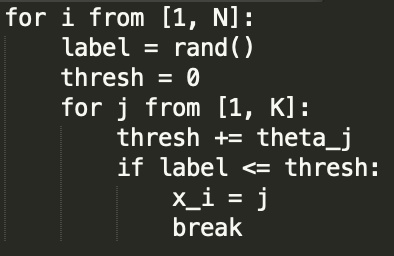
\includegraphics[scale=0.5]{code1.png} This pseudocode should work as long as all the thetas add up to 1.

\item Write a function (in whatever language you prefer, e.g., Matlab, Python, R, etc)  that takes as input the parameters of a Dirichlet distribution with $K=3$, i.e., $Dir(\alpha_1, \alpha_2, \alpha_3)$ and generates a contour plot of the Dirichlet density function (with these parameter values) over the 2-dimensional simplex where the  simplex has $\alpha_1$ as the x-axis and $\alpha_2$ as the y-axis. You do not need to write your own function for generating contours: you should be able to find a plotting function to do this in whatever language you are using.
Using your code generate plots that show:
\begin{enumerate}
\item  A prior defined as $Dir(4,4, 4)$ 
\item  The posterior density with $Dir(4,4, 4)$ as the prior and with $N=20$ data points simulated from a multinomial with $\theta_1 = 0.1, \theta_2 = 0.5, \theta_3 = 0.4$. 
\item The posterior density with the same prior and data from the same multinomial but now with $N=200$ data points.
\end{enumerate}
Use your solution from part 1 to write code to simulate the data points.   Submit the 3 plots above. No need to submit your code.

\item Now repeat the previous part of this question but with a prior defined as $Dir(50,10,40)$. Submit the 3 plots again and write a few sentences comparing the two sets of 3 plots  (with the two different priors).

 \end{enumerate}

 


\end{document}